\section{Modeling a reinsurance company financial structure}
\label{sec:COMPANY_DESCRIPTION}

A reinsurance group est generally composed of several independent companies that are called "legal entities". These companies are subsidiaries of a mother company (or subsidiaries of subsidiaries), and not branches : each of them has regulatory requirements depending of the country in which they are incorporated. This is not the case of branches that are only extensions of their mother company.

\subsection{Ownership structure}
\label{sec:OWNERSHIP}


A hierarchical ownership structure is almost always chosen. (This allows to reduce fiscal losses during the dividends "ascent" to the mother company and the shareholders). The word "Group" is used to describe all companies directly or indirectly owned by the parent company including itself).

An example of ownership structure in given in \ref{fig:GROUP_STRUCTURE}. Black arrows represent the ownership links and a hierarchical structure is chosen in this example.

\begin{figure}
\centering
  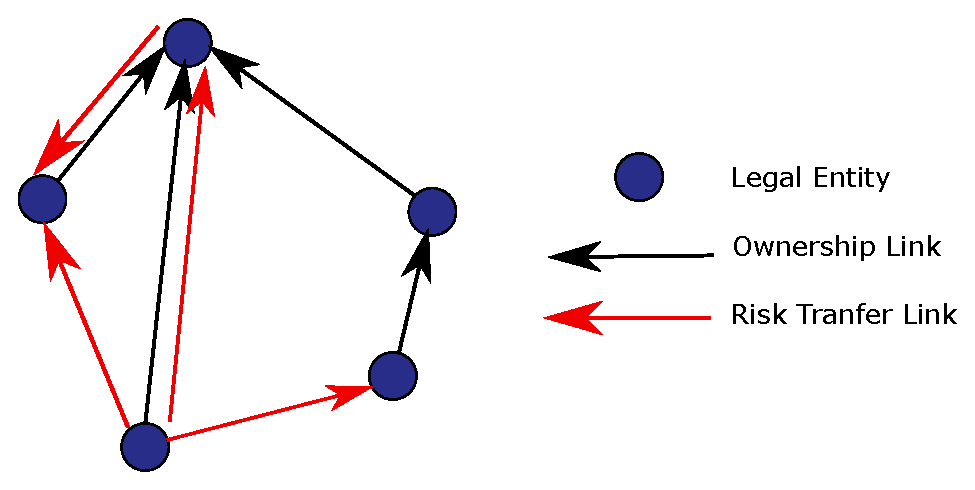
\includegraphics[width=\linewidth]{images/part1/group_structure.eps}
  \caption{Representation of the (black arrow) ownership structure (arrow means "belong to") and (red arrow) risk transfer structure (arrow means "transfer risk to") of a (re)insurance group. Legal entities are represented as blue disks.}
  \label{fig:GROUP_STRUCTURE}
\end{figure}



\subsubsection{Financial statements representation}
\label{sec:FINANCIAL_STATEMENT}

Each legal entity must disclose financial statements to its regulator. These financial statements contain at least :
\begin{itemize}
  \item a balance sheet,
  \item a profit and loss statement,
\end{itemize}
(what about the cash flow statement?). The balance sheet display the assets and liabilities of the company, which are always equal at any given time. 
For the purpose of stress testing scenarios, only the balance sheet is considered. Indeed, the balance sheet is a representation of the company patrimony at a given time, and the solvency of an insurance company is assessed by comparing the capital on the balance sheet with a regulatory required capital. But this do not allow to easily visualize changes in premium income or charges.

\begin{figure}[h!]
\centering
  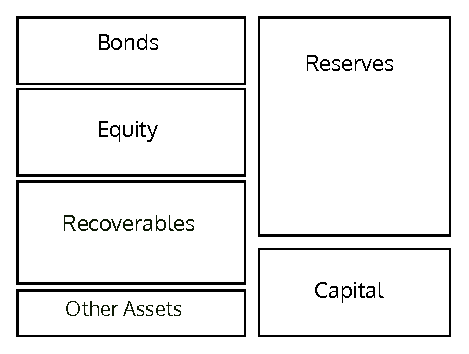
\includegraphics[width=70mm]{images/part1/balancesheet.eps}
  \caption{Simplified representation of a balance sheet.}
  \label{fig:BALANCE_SHEET}
\end{figure}


This representation of the balance sheet is a simplified one, but these elements will be enough for the next step of the report to understand the dynamic of operation of a reinsurance company. It is important to understand that the wealth of the shareholders of the company correspond to the company "Own Funds", also called "Capital". More information on the variation of balance sheet values due to a shock are given in section \ref{sec:BS_SHOCK}.

Moreover, each legal entity is characterized by its own balance sheet, and in this work, we will assume that the group balance sheet is the sum of all legal entities balance sheets.

JUSTIFY THIS ASSUMPTION

\begin{figure}[h!]
\centering
  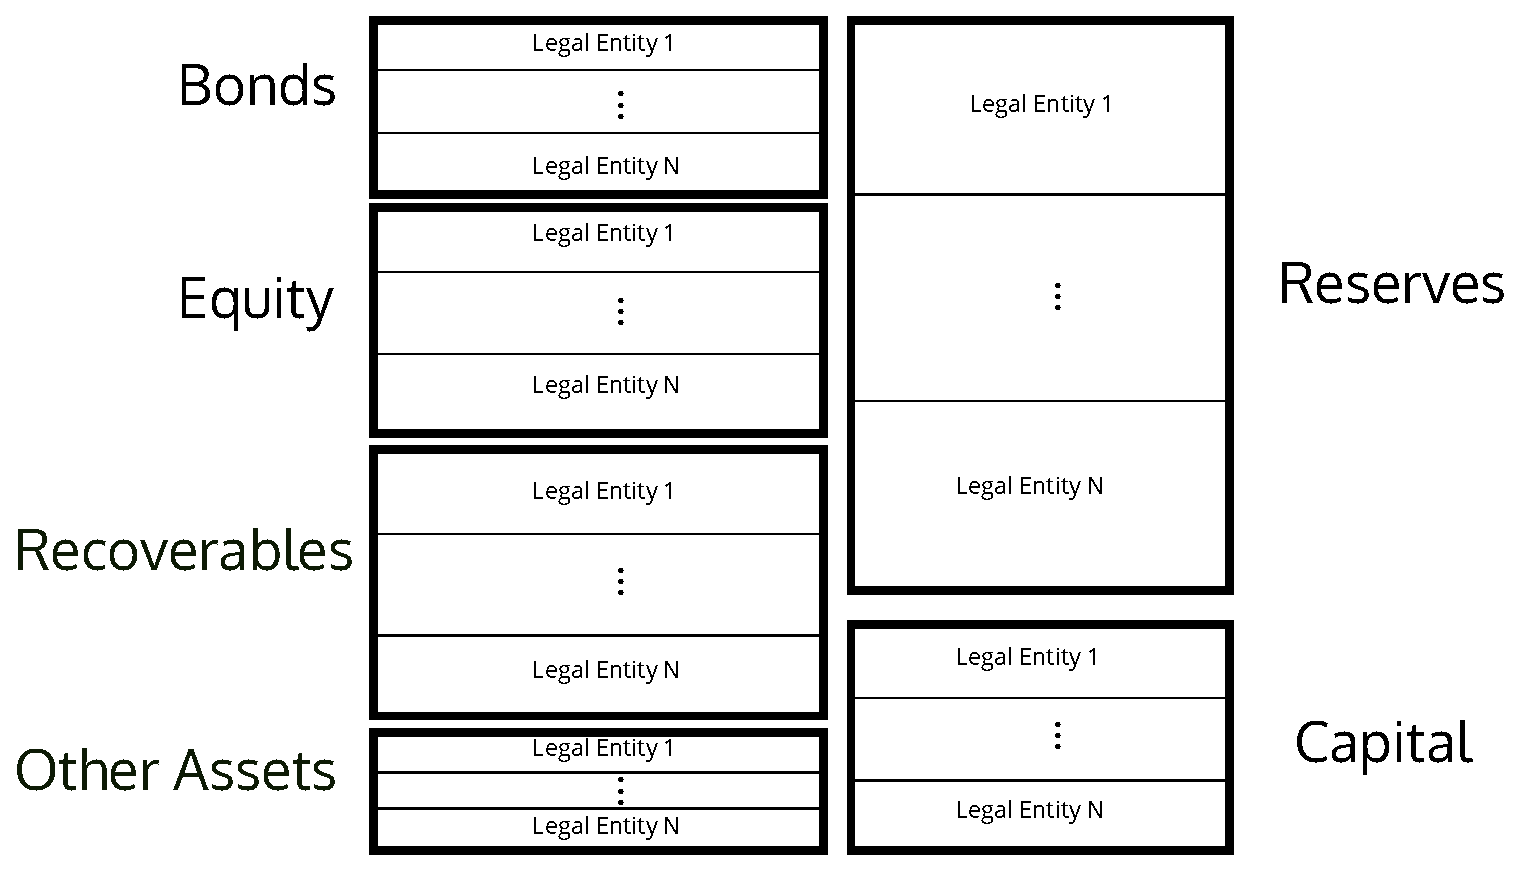
\includegraphics[width=120mm]{images/part1/agreg_balance_sheets.eps}
  \caption{Aggregation of legal entities balance sheets into the group balance sheet.}
  \label{fig:BALANCE_SHEET}
\end{figure}


From a mathematical point of view, a re-insurance group can composed of $N$ legal entities, each of them having a $C_i$, $i$ being the ith entity. All legal entities capitals are summarized by the vector:

\begin{equation}
    C = (C_i)_{i \in [1, N]}
\end{equation}


This vector can be splitted into several components related to the balance sheet :

\begin{equation}
    C = FI + E + Recov + OA - Res
    \label{eq:CAPITAL_DEF}
\end{equation}

with $FI$ the fixed Income (Bonds) vector, $E$ the equity vector, $Recov$ the recoverable vector, $OA$ the other asset vector and $Res$ the reserve vector.


\subsubsection{Exposure of legal entities}
\label{sec:EXPOSURE_DEF}

Each legal entity has its own financial position and risk profile, determined by the nature of the risks it underwrites. The exposure of a company is defined by the level of its liabilities toward policyholders per geographic zones and lines of businesses. For instance, a company underwriting natural catastrophe business in the USA is highly exposed to a hurricane on Florida but absolutely not to a deviation of life expectancy in China. 
This notion of exposure is important as it represents the "entry points" of losses within the company. One can visualize the exposure as a target whose area proportional to the liabilities of a company. Within a reinsurance group, each legal entity can have very different exposures, and ultimately, each legal entity is liable to the risks it underwrites.

From a mathematical point of view, each legal entity can suffer a loss $L_i$, $i$ being the ith entity. Losses on all legal entities are summarized by the vector:

\begin{equation}
    L = (L_i)_{i \in [1, N]}
\end{equation}
